
\section*{STRIDE: Microsoft’s Threat Modeling Framework}
STRIDE is a mnemonic framework developed by Microsoft to systematically identify and categorize security threats in software systems\cite{shostack2014}. Each letter represents a distinct threat category:
\begin{itemize}
	\item \textbf{S}poofing identity: Illegitimate access by pretending to be another user or system.
	\item \textbf{T}ampering with data: Unauthorized modification of data or code.
	\item \textbf{R}epudiation: Denial of actions or transactions by users, often due to lack of proper logging.
	\item \textbf{I}nformation disclosure: Unauthorized exposure of sensitive information.
	\item \textbf{D}enial of service: Disruption of service availability to legitimate users.
	\item \textbf{E}levation of privilege: Gaining higher access rights than intended.
\end{itemize}

\subsection*{Technical Definitions and Application}
	extbf{Spoofing:} The act of pretending to be someone or something else to gain unauthorized access. Example: Using stolen credentials to log in as another user.\cite{shostack2014}

	extbf{Tampering:} Unauthorized alteration of data or code, such as modifying a database record via SQL injection.\cite{owasp}

	extbf{Repudiation:} The ability of users to deny their actions, often due to insufficient logging or lack of digital signatures.\cite{nist800154}

	extbf{Information Disclosure:} Accidental or malicious exposure of confidential data, such as leaking PII through misconfigured APIs.\cite{uceda2015}

	extbf{Denial of Service:} Attacks that disrupt the availability of a service, e.g., DDoS attacks on login endpoints.\cite{owasp}

	extbf{Elevation of Privilege:} Exploiting vulnerabilities to gain higher access, such as exploiting a vulnerable admin panel.\cite{shostack2014}

\subsection*{STRIDE Threat Categories Table}
\begin{table}[H]
\centering
\begin{tabular}{|l|l|l|l|}
\hline
	extbf{Category} & \textbf{Description} & \textbf{Example} & \textbf{Control} \\
\hline
Spoofing & Impersonating users or systems & Stolen credentials & MFA, strong auth \\
Tampering & Modifying data or code & SQL injection & Input validation, hashing \\
Repudiation & Denying actions & Log deletion & Audit logs, digital signatures \\
Information Disclosure & Leaking sensitive data & Data breach & Encryption, access control \\
Denial of Service & Disrupting service & DDoS attack & Rate limiting, WAF \\
Elevation of Privilege & Gaining unauthorized access & Privilege escalation & RBAC, least privilege \\
\hline
\end{tabular}
\caption{STRIDE Threat Categories, Examples, and Controls\cite{shostack2014,owasp}}
\end{table}

\subsection*{STRIDE and Data Flow Diagrams (DFDs)}
STRIDE is most effective when applied to Data Flow Diagrams (DFDs), which visually represent system components, data stores, and trust boundaries. Each element is analyzed for threats in all STRIDE categories.\cite{shostack2014}

\begin{figure}[H]
	\centering
	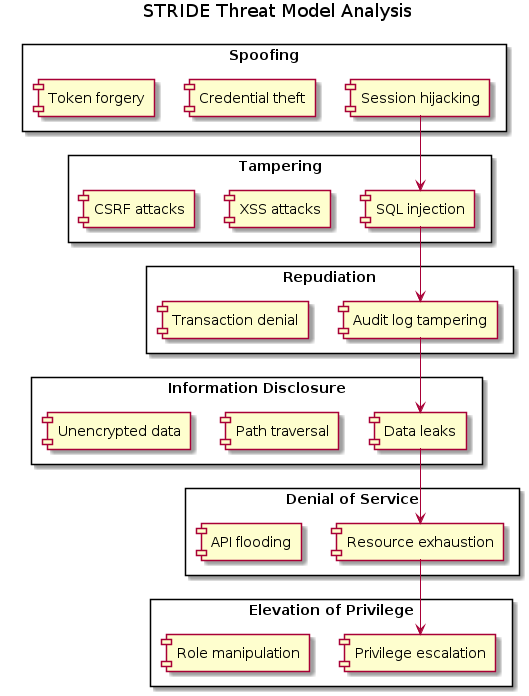
\includegraphics[width=0.7\textwidth]{images/stride-analysis}
	\caption{Example STRIDE Analysis on a Data Flow Diagram}
\end{figure}

\subsection*{Practical Example}
Consider a web application with user authentication, a database, and an admin panel. Applying STRIDE:
\begin{itemize}
	\item \textbf{Spoofing:} Attackers use phishing or credential stuffing to impersonate users.
	\item \textbf{Tampering:} SQL injection to alter database records.
	\item \textbf{Repudiation:} Users delete logs to hide malicious actions.
	\item \textbf{Information Disclosure:} Sensitive data exposed via misconfigured APIs.
	\item \textbf{Denial of Service:} Attackers flood the login endpoint.
	\item \textbf{Elevation of Privilege:} Exploiting a vulnerable admin panel to gain root access.
\end{itemize}

\subsection*{STRIDE in Secure Development}
Microsoft recommends integrating STRIDE into the Secure Development Lifecycle (SDL), using it to drive security requirements, code reviews, and testing. Modern tools, such as the Microsoft Threat Modeling Tool, automate parts of the STRIDE process and help teams visualize threats and mitigations\cite{shostack2014,owasp}.
